\chapter{Datengrundlage}
\label{chap:datengrundlage}
Das Ziel der Anwendung liegt in der Darstellung von Modelldaten durch das \kps innerhalb der realen Umgebung. Dazu soll in diesem Kapitel eine geeignete Modellstruktur definiert. Als Grundlage für die spätere Lokalisation ist es erforderlich, ein möglichst originalgetreues Abbild der realen Umgebung zu erstellen. Eine hohe Modellgüte ermöglicht den Abgleich zwischen Modell- und Umgebungsdaten und erlaubt die präzise Positionierung virtueller Objekte sowohl in der Modell-\red[Modellumgebung oder Modell-Umgebung?] als auch in der realen Umgebung. Die in der realen Umgebung zu visualisierenden Modellobjekte werden auf Basis der virtuellen Umgebungsdaten erstellt und positioniert. Die Projektion der Modellumgebung selbst innerhalb der realen Umgebung würde lediglich zu Überlagerungen gleicher Strukturen führen und besitzt außerhalb von Validierungen des \kps{s} keine Relevanz.\\

\section{Modellumgebung}
Für die Verwendung der erstellten Programmstruktur ist es erforderlich, dass die Umgebung in Form eines 3D Modells abgebildet wird. Als Modellumgebung werden dabei alle statischen Objekte und Strukturen betrachtet, welche eine Repräsentation der realen Umgebung darstellen. Um die benötigten Daten zu generieren können verschiedene Verfahren angewendet werden.\\
Liegen bereits Modelldaten der Umgebung vor, so kann das virtuelle Umgebungsmodell direkt aus diesen abgeleitet werden. Insbesondere ist dies der Fall, wenn die Anwendung des \kps{s} in die Planungs- und Bauphase eines Gebäudes integriert werden soll. Eine beispielhafte Modellumgebung ist in \abb{fig.mapMod} dargestellt.\\

\begin{figure}[ht]
	\begin{center}
		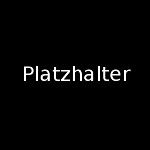
\includegraphics[scale=1.0]{spacer}
		\caption{Karte Modell}
		\label{fig.mapMod}
	\end{center}
	%\vspace*{-8mm}
\end{figure}


Für den Einsatz des \kps{s} ohne vorhandene aktuelle Modelldaten kann eine Kartierung \red[(Mapping)] der Umgebung erfolgen. Die Kartierung von 2D- und 3D-Umgebungen ist in aktuellen Forschungen eng mit der Lokalisation innerhalb dieser Umgebungen verknüpft. Ein verbreitetes Forschungsfeld in diesem Zusammenhang ist das simultane Kartieren und Lokalisieren in unbekannten Umgebungen (engl. \textit{Simultaneous Localization And Mapping}, kurz SLAM). Dabei existieren verschiedene Algorithmen und Implementierungen zur Lösung der Problemstellungen. Die Kartierung selbst soll in dieser Arbeit nicht näher erläutert werden, für eine detailliertere Darstellung sei deshalb auf \red[\cite{Durrant2006}] verwiesen.\\
Zur Validierung des Systems wurde die in \abb{fig.mapSLAM} dargestellte Umgebung aufgezeichnet. Dabei wurde eine Implementierung \cite{Rgbdslam} nach Endres \textit{et al.} \cite{Endres2014} verwendet. Da diese die Kartierung mittels einer RGB-D Kamera ermöglich, ist der Einsatz des \kps{} auch in diesem Schritt möglich.

\begin{figure}[ht]
	\begin{center}
		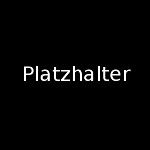
\includegraphics[scale=1.0]{spacer}
		\caption{Karte RGBDSLAM Subfigures: echter raum (?) - Punktewolke}
		\label{fig.mapSLAM}
	\end{center}
	%\vspace*{-8mm}
\end{figure}

%Boingboingboingboingboingboingboingboingboingboing. Boing?
Das Ergebnis der Kartierung entspricht einer texturierten Punktwolke. Im Gegensatz zu der Ableitung aus vorhandenen Modelldaten handelt es sich daher nicht um geschlossene Geometrien. Da die Umgebung selbst jedoch ohnehin nicht als Teil der Projektion eingesetzt wird hat dies keine Auswirkungen auf die Funktionalität des Systems. Nachteiligen Einfluss können jedoch die im Vergleich zu Modelldaten geringere Auflösung sowie die Rauscheinflüsse des Kinect-Sensors zeigen. Die Güte eines Modells aus der Kartierung liegt deshalb meist unter der Modellgüte bei Ableitung aus vorhandenen 3D-Daten. Durch Verwendung der selben Sensoren während der Kartierung und der Lokalisation können die Fehlereinflüsse jedoch leicht verringert werden, da sich wiederholende Sensoreinflüsse so bei beiden Verfahren auftreten.\\

\section{Modellobjekte}
Für die Projektion der visuellen Zusatzinformationen sind zu Grunde liegende Modelldaten erforderlich. Modellobjekte beschreiben somit alle Strukturen und Objekte, welche keine Elemente der realen Umgebung abbilden. Die zur Erstellung der Modellumgebung beschriebenen Verfahren können dabei ebenso auf die Modellierung von Objekten und Strukturen angewendet werden. Anstelle von Algortihmen zur Kartierung der Umgebung könnten dabei jedoch spezielle Verfahren zur Erfassung dreidimensionaler Objekte eingesetzt werden, wie beispielsweise von \cite{Xu2012} beschrieben.\\
Die Modellobjekte müssen anders als die Modellumgebung jedoch nicht als reale Objekte vorhanden sein, weshalb sie auch keine Auswirkungen auf die Lokalisation haben. Es können somit beliebige Objekte modelliert werden um diese später in der realen Umgebung zu visualisieren.\\
Die Modellgüte hat in allen Fällen keine Auswirkungen auf die Lokalisations- oder Projektionsgenauigkeit. Für die Visualisierung ist jedoch eine ausreichende Auflösung der Modellstrukturen und -texturen anzustreben.\\

\section{Dateistruktur}
Um die Szene, bestehend aus der Modellumgebung und allen integrierten Modellobjekten, später wieder in den virtuellen Planungsablauf integrieren zu können wird eine Dateistruktur definiert, welche die Sicherung der aktuellen Modellkonfiguration ermöglicht. Alle Modellelement werden dazu mit ihrer aktuellen Pose, Textur und geometrischen Repräsentation erfasst und aufgezeichnet. Eine Wiederherstellung verschiedener Konfigurationen ist damit ebenfalls jederzeit möglich.\\
\red[Dateiformat? Eine Datei enthält alle Informationen über die Welt und über die einfügbaren Objekte (Preview Funktion). Hinzufügen/entfernen von Objekten zur Datei möglich, suchen nach vorhandenen Objekten in Datenbank möglich?]